\documentclass[a4paper, 11pt, oneside]{report} 
\usepackage[utf8]{inputenc}
\usepackage[dutch]{babel}
\usepackage{amsmath}
\usepackage{amsfonts}
\usepackage{amssymb}
\usepackage{graphicx}
\usepackage{caption}
\usepackage[table,xcdraw]{xcolor}
\usepackage[toc,page]{appendix}
\usepackage{hyperref}
\usepackage{titlesec}
\usepackage{listings}
\usepackage{float}
\usepackage{tikz}
\usetikzlibrary{trees}
\usepackage{tikz-qtree}
\usepackage{graphicx}
\usepackage{fancyref}
\usepackage{wrapfig}
\usepackage{url}
\usepackage{pdflscape}
\usepackage{fancyvrb}
\usepackage{fancyhdr}
\graphicspath{ {Afbeeldingen/} }
\usepackage{subfig}
\usepackage{tabularx}
\usepackage{apacite}
\usepackage{longtable}
\usepackage{titlecaps}
%\usepackage[T1]{fontenc}
\usepackage{titlesec, blindtext, color}
\definecolor{gray75}{gray}{0.75}
\newcommand{\hsp}{\hspace{20pt}}
\usepackage{pdfpages}
\usepackage{siunitx}
\sisetup{per-mode=symbol,binary-units=true } 

\newcolumntype{L}[1]{>{\raggedright\arraybackslash}p{#1}}

\titleformat{\chapter}[hang]{\huge\bfseries}{\thechapter\hsp\textcolor{gray75}{|}\hsp}{0pt}{\Large\bfseries}

\def\figureautorefname{Figuur}
\def\sectionautorefname{Paragraaf}
\def\chapterautorefname{Hoofdstuk}
\def\tableautorefname{Tabel}
\DeclareRobustCommand{\VAN}[3]{#2} % set up for citation

%% Sets page size and margins 
\usepackage[a4paper,top=3cm,bottom=3cm,left=3cm,right=3cm,marginparwidth=1.75cm]{geometry}

\author{M.W.J. Berentsen}
\font\myfont=cmr12 at 40pt
\title{\myfont Drone meshnetwerk simulatie}
\usepackage{titling}

\newcommand{\subtitle}[9]{%
	\posttitle{%
		\par\end{center}
	\begin{center}\large#1\end{center}
	\begin{center}\large#2\end{center}
	\vskip0.5em
	\begin{center}\normalsize#3\end{center}
	\begin{center}\large#4\end{center}
	\begin{center}\large#5\end{center}
	\begin{center}\large#6\end{center}
	\begin{center}\normalsize#7\end{center}
	\begin{center}\normalsize#8\end{center}
	\begin{center}\normalsize#9\end{center}
	\vskip0.5em}%
	\rfoot{{\footnotesize \textbf{#1}}}
}

\subtitle{Software Requirement Specificatie}{Versie 2.0}{Alten Nederland B.V.}{Hogeschool van Arnhem en Nijmegen}{HBO Technische Informatica - Embedded Software Developement }{MWJ.Berentsen@student.han.nl}{Studentnummer: 561399}{Docent: J. Visch, MSc}{Assessor: ir. C.G.R. van Uffelen}

\setlength{\parindent}{0pt}
\setlength{\parskip}{5pt plus 2pt minus 1pt}



\hypersetup{colorlinks=true, urlcolor=red,citecolor=black,linkcolor=blue}  % Colours hyperlinks in blue, but this can be distracting if there are many links.
\setcounter{tocdepth}{2}

\usepackage{fancyhdr}
\pagestyle{fancy}

\setlength\headheight{26pt} %% just to make warning go away. Adjust the value after looking into the warning.
% \rhead{{\color{blue}\rule{1cm}{1cm}}}

\rhead{
\includegraphics[height=1cm]{Afbeeldingen/han.png}}



\begin{document}
\begin{figure}
\begin{center}
\includegraphics[scale=0.1]{alten}\end{center}
\end{figure}
\maketitle

%\section*{Voorwoord}
%\addcontentsline{toc}{section}{\protect\numberline{}Voorwoord}
%\pagebreak

%Geschikt voor minimaal 50 nodes; Kan slecht of geen signaal nabootsen

\tableofcontents
\clearpage
%\section*{Begrippenlijst}

% Please add the following required packages to your document preamble:
% \usepackage[table,xcdraw]{xcolor}
% If you use beamer only pass "xcolor=table" option, i.e. \documentclass[xcolor=table]{beamer}
%\begin{table}[H]
%\centering

\chapter*{Begrippenlijst}
\label{inleiding:begrippenlijst}

\begin{longtable}[c]{|l|l|}
	\hline
	\rowcolor[HTML]{9B9B9B} 
	Term & Beschrijving \\ \hline
	\endhead
	%
	Byte & Een samenstelling van 8 bits. \\ \hline
	Gazebo & Simulatiesoftware met ondersteuning voor physics. \\ \hline
	nRF24l01+ & Radio transciever module werkzaam op de 2,4Ghz band. \\ \hline
	Physics engine & Software die natuurwetten toepast op virtuele objecten. \\ \hline
	\begin{tabular}[c]{@{}l@{}}Raspeberry Pi \\ model 2B+\end{tabular} & Micro computer geschikt voor prototyping. \\ \hline
	Ros & \begin{tabular}[c]{@{}l@{}}Robot operating system. Wordt gebruikt voor de transportlaag \\ naar zowel virtuele als gesimuleerde robots.\end{tabular} \\ \hline
	Router & Netwerkcomponent die berichten kan doorsturen. \\ \hline
	Seriële verbinding & Een communicatieverbinding bekend van USB en RS232. \\ \hline
	Simulatie software & Software die fysieke objecten nabootst in software. \\ \hline
	Unittest & Geautomatiseerde test die functie test op resultaat. \\ \hline
	\caption{Begrippenlijst.}
	\label{tab:begrippenlijst}\\
\end{longtable}

%\clearpage

%\section*{Samenvatting}
%\addcontentsline{toc}{section}{\protect\numberline{}Samenvatting}
%\pagebreak


\chapter{Inleiding}
\label{inleiding}
\section{Algemene beschrijving}
\label{inleiding:beschrijving}
Het volgende verslag betreft de Software Requirements Specification voor de afstudeerstage van Maurice Berentsen (hierna: student).
Dit document volgt het document: \textit{``Software Requirements Specification Template``} \cite{template:srs}.

Het doel van dit project is het zetten van de eerste stap in de ontwikkeling van het dronenetwerk.
De eerste stap is ontwikkelen van een netwerkmodule voor het onderling verbinden van drones.
Het is van belang dat het meshnetwerk van de drones snel kan reageren op uitval van netwerkpunten.
Deze netwerkmodule moet zowel virtueel als fysiek gerealiseerd worden in dit project.
 

\section{Doel van dit document}
\label{inleiding:doelvanditdoucment}

In dit document zullen de gebruikers, eisen en usecases van het systeem beschreven worden zodat het duidelijk is wie gebruik gaat maken van het systeem en welke functionaliteiten het systeem bevat.   

\section{Actoren en hun eigenschappen}
\label{inleiding:gebruikers}
In dit deel worden de actoren van het systeem omschreven. 
Elke actor wordt kort omgeschreven per paragraaf.

\subsection{Dronecontroller}
\label{inleiding:gebruikers:dronecontroller}
Een dronecontroller is de gebruiker die het systeem wil gebruiken om drones naar plekken toe te kunnen sturen.
Hij wil hiermee een netwerk van onderling verbonden drones uitzetten.  

\subsection{Netwerkgebruiker}
\label{inleiding:gebruikers:netwerkgebruiker}
Een netwerkgebruiker wil het netwerk gebruiken om data te kunnen versturen naar een andere punt binnen of buiten het netwerk. 

\subsection{Algoritmetester}
\label{inleiding:gebruikers:algoritmetester}
Een algoritmetester wil het netwerk gebruiken om de verdeling van drones te kunnen analyseren om tot een zo goed mogelijk verdeelalgoritme te komen.

\section{Werkomgeving}
\label{inleiding:werkomgeving}
Deze paragraaf omschrijft zowel de hardware- als softwareomgeving waarin dit project wordt uitgevoerd. 

\subsection{Ubuntu 18.04.2 LTS}
\label{inleiding:werkomgeving:ubuntu}
In het project wordt gebruik gemaakt van Ubuntu 18.04.2 LTS vanwege de ondersteuning die het biedt voor \nameref{inleiding:werkomgeving:ros}.
Hoewel er een versie van ros opkomend is voor Windows zal hier op het moment geen rekening mee gehouden worden.
De opgeleverde code wordt ontwikkeld en gecompileerd op een Ubuntu machine.


\subsection{Raspberry Pi model B+}
\label{inleiding:werkomgeving:raspberrypi}

In het project wordt gebruik gemaakt van een Raspberry Pi als prototype board.
Deze microcomputer is voorzien van een Broadcom BCM2836 SoC en heeft een 40 pin General Purpose Input Output (GPIO).
Hiervan zijn 27 pinnen beschikbaar voor input, output maar ook geavanceerde technieken als PWM, SPI, I2C  of een seriële verbinding.
Verder biedt het twee 3,3 en twee 5 volt aansluitpunten aan.


\subsection{NRF24}
\label{inleiding:werkomgeving:nrf24}
De NRF24 is gekozen door zijn prestaties ten opzichte van afstand.
De mogelijkheid om een snelheid aan te kunnen bieden van \SI{250}{\kilo\bit\per\second} op een afstand van 500 meter maakt deze module het meest geschikt voor dit project.
Daarnaast kan de NRF24 tot zes adressen tegelijk onderhouden die kunnen schakelen tussen zenden en ontvangen.
De NRF24 is in staat om per payload tot 32 bytes te versturen. 
Tenslotte is de NRF24 een transciever die werkt op een voltage van 3.3 volt waarbij de I/O pinnen 5 volt tolerant zijn wat het compatibel maakt met de \nameref{inleiding:werkomgeving:raspberrypi}.

\subsection{Drone}
\label{inleiding:werkomgeving:drone}
Hoewel in dit project drones een onmisbaar onderdeel zijn wordt er niet gesproken over een specifiek merk of type drone.
De reden hiervoor is, omdat er geen focus ligt op een specifieke drone, en de student ook niet gecertificeerd is om te vliegen met zakelijke drones.
Er zal gewerkt worden met gesimuleerde drones. 
Deze hebben een interface die in staat is om een drone te laten vliegen naar een specifiek coördinaat en de huidige locatie aan te geven.

\subsection{ROS}
\label{inleiding:werkomgeving:ros}
ROS is middleware software die gebruikt wordt voor de aansturing en simulatie van robotica. 
In het geval van dit project wordt ROS gebruikt voor de communicatie naar de \nameref{inleiding:werkomgeving:drone} toe, maar ook voor het simuleren van de \nameref{inleiding:werkomgeving:nrf24} communicatie tussen de drones. 

\subsection{Gazebo}
\label{inleiding:werkomgeving:gazebo}

Gazebo is een opensource robot simulatie framework bijzonder geschikt voor het simuleren van robotica in outdoor omgevingen door de uitgebreide Physics Engine Support \cite{gazebo}.
In dit project wordt nu geen gebruik gemaakt van de physics engine. Doordat de netwerkonderdelen als virtuele onderdelen beschikbaar zijn in gazebo kunnen ze aangesloten worden op een gesimuleerde drones die wel realistisch vlieggedrag vertonen.
Deze mogelijkheid was daarom ook een hoofdreden om Gazebo te gebruiken.

\subsection{Catkin}
\label{inleiding:werkomgeving:catkin}

Catkin is de ingebouwde standaard build tool van ROS. De tool is een combinatie van CMake en door ROS geschreven python scripts \cite{catkin}. Deze wordt gebruikt in het project om de simulatiesoftware mee te bouwen. 


\subsection{Gtest (Google unittest)}
\label{inleiding:werkomgeving:gtest}

Google test wordt gebruik voor het schrijven van unit testen binnen ROS \cite{googletest}. Omdat het gebruik van Gtest erg populair is binnen de ROS community maat dit het identificeren van problemen makkelijker maakt. 




\section{Ontwerp en implementatie beperkingen}
\label{inleiding:ontwerpberkingen}

De software wordt ontwikkelt in een ROS omgeving hiervoor worden de volgende eisen gesteld:
\begin{itemize}
	\item  Zie \href{http://wiki.ros.org/ROS/Introduction\#Operating\_Systems}{http://wiki.ros.org/ROS/Introduction\#Operating\textunderscore Systems} voor ondersteuning van platformen. ROS draait op een Unix-based platform.
	\item De software dat voor het project is ontwikkelt, is op Ubuntu 18.04 gemaakt, aangeraden is dus ook om dit te gebruiken.
\end{itemize}

Om de drones te kunnen simuleren is er voor gekozen om gebruik te maken van Gazebo hierbij worden de volgende hardware eisen gesteld:

\begin{itemize}
	\item Een GPU die werkt met OpenGL 3D accelerated driver.
	\item Een CPU welk op zijn minst een Intel i5 is of vergelijkbaar \cite{gazeborequirements}. 
	\item Op zijn minst 500 MB vrije opslag ruimte.
\end{itemize}


\section{Product Functies}
\label{inleiding:productfuncties}
In het onderstaande diagram \ref{fig:usecasediagram} is te zien wie er betrokken is bij het systeem(actoren) en hoe ze het systeem gebruiken om hun doel te bereiken.
Een netwerkgebruiker is maar geïnteresseerd in één usecase, hij wil namelijk alleen gebruik maken van het netwerk om zijn data te versturen.
De dronecontroller wil een dronenetwerk kunnen ontplooien en drones verzoeken om te verplaatsen.
Een algoritmetester wil het dronenetwerk simuleren en wil daarom alleen die usecase uitvoeren.
Deze usecase kan wel gebruik maken van dezelfde usecases als een dronecontroller maar doet dat dus in een gesimuleerde omgeving. 
\begin{figure}[H]
	\begin{center}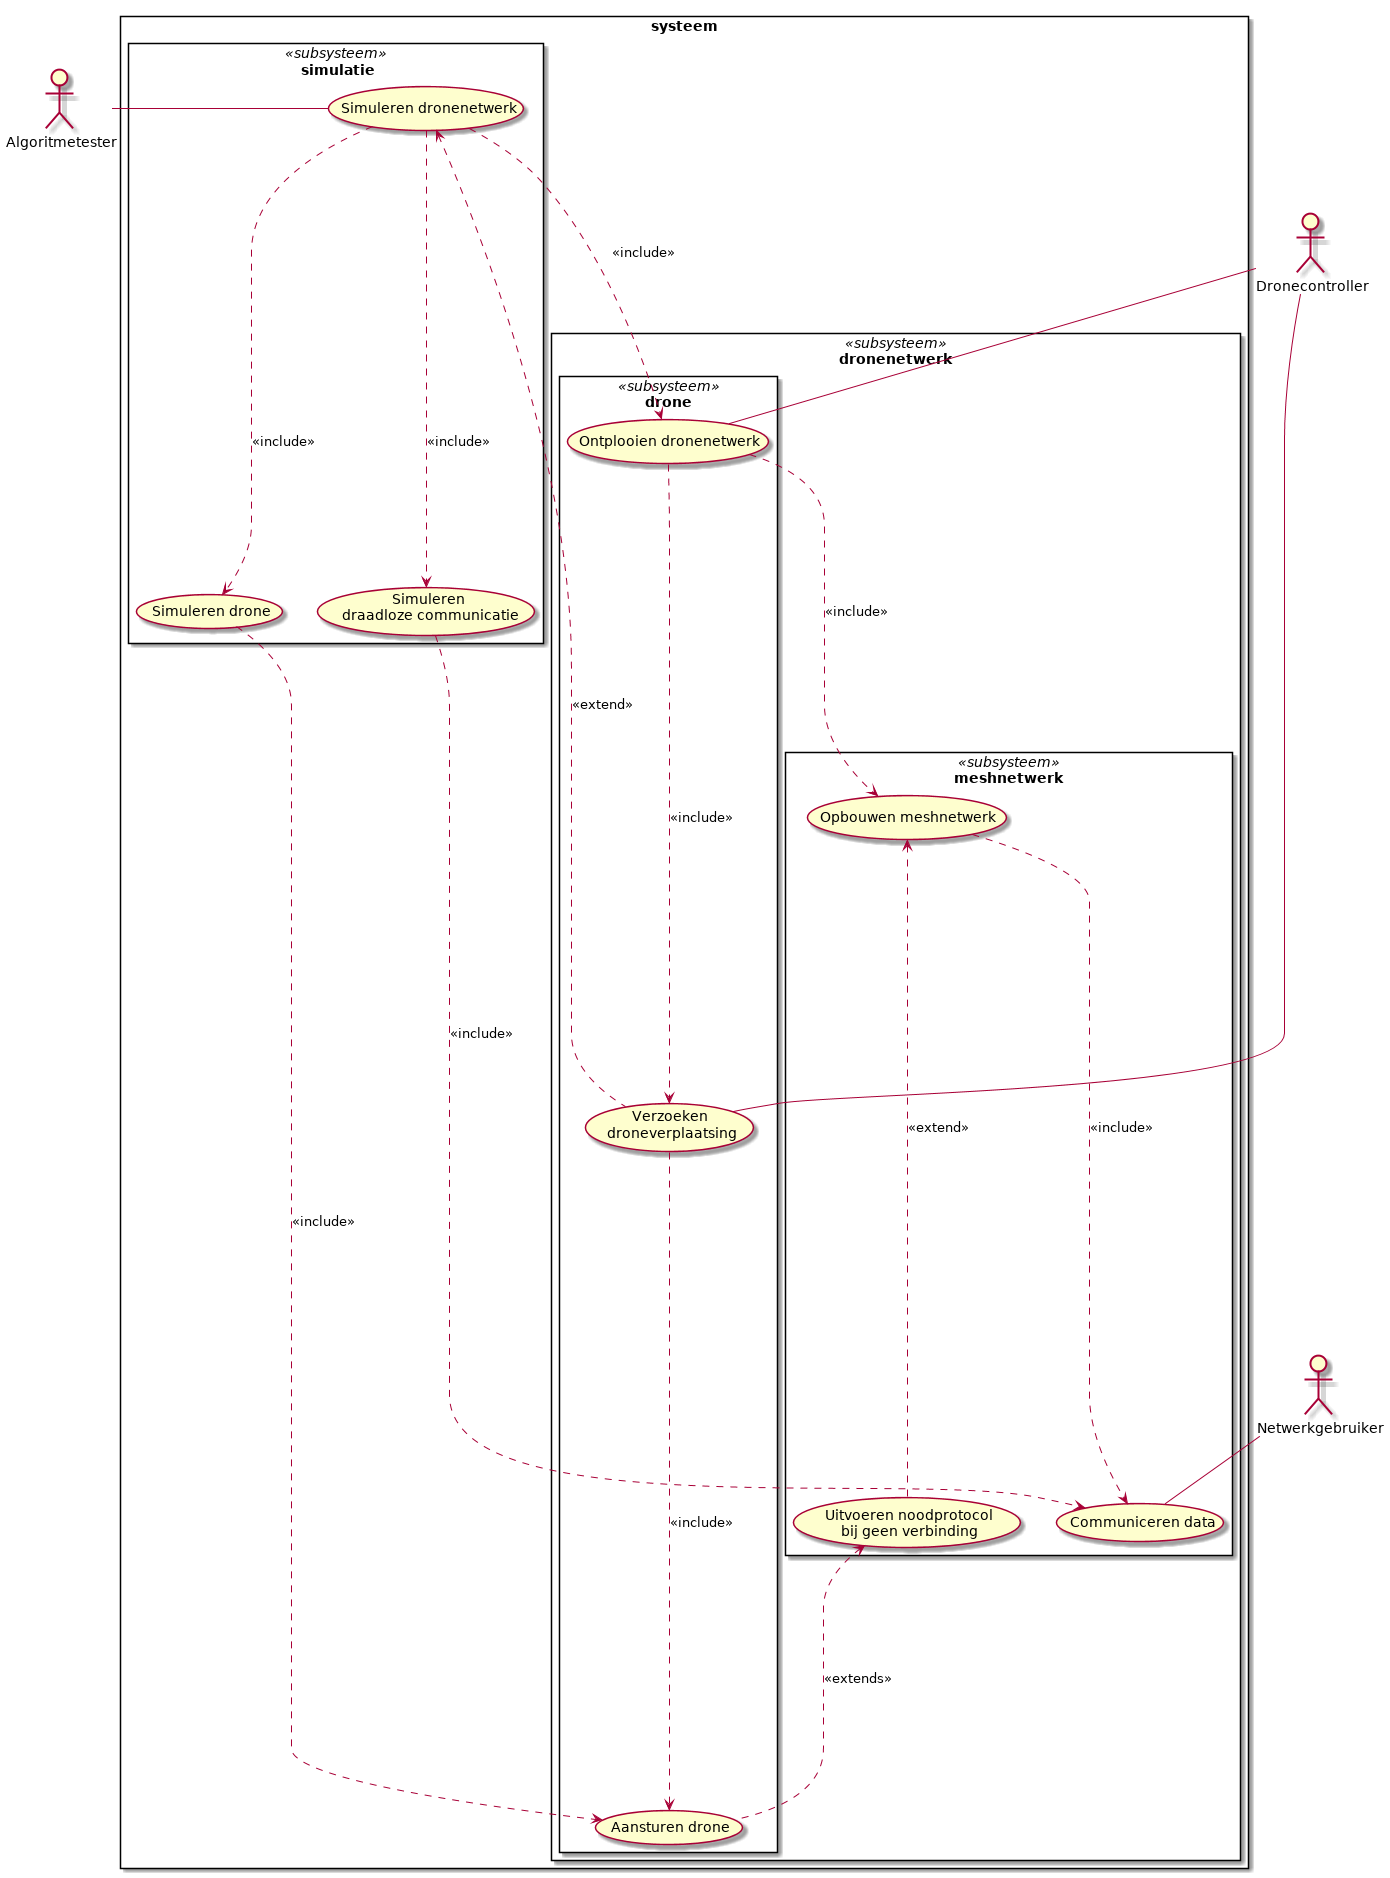
\includegraphics[width=1\linewidth]{UML/out/usecase/usecasediagram/usecasediagram.png}\end{center}
	\caption{Usecase diagram.}
	\label{fig:usecasediagram}
\end{figure}

\begin{table}[H]
	\centering
	\begin{tabular}{|l|l|}
		\hline
		\rowcolor[HTML]{C0C0C0} 
		Usecase & Beschrijving \\ \hline
		\nameref{Usecase:simulatiedronenetwerk} & \begin{tabular}[c]{@{}l@{}}Een actor wil een dronenetwerk simuleren. Hiervoor moeten\\ drones en draadloze communicatie gesimuleerd worden.\end{tabular} \\ \hline
		\nameref{Usecase:simulatiedrone} & Het systeem gaat een drone simuleren. \\ \hline
		\hyperlink{draadlozecom}{\begin{tabular}[c]{@{}l@{}}Simuleren draadloze \\ communicatie\end{tabular}} & \begin{tabular}[c]{@{}l@{}}Het systeem gaat draadloze communicatie simuleren. \\ Hiermee kan het data communiceren.\end{tabular} \\ \hline
		\nameref{Usecase:communicerendata} & \begin{tabular}[c]{@{}l@{}}Een actor geeft aan dat hij data wil communiceren via het\\ netwerk.\end{tabular} \\ \hline
		\nameref{Usecase:opbouwenmeshnetwerk} & \begin{tabular}[c]{@{}l@{}}Het systeem gaat een meshnetwerk opbouwen tussen \\ aanwezige nodes.\end{tabular} \\ \hline
		\hyperlink{noodprotocol}{\begin{tabular}[c]{@{}l@{}}Uitvoeren noodprotocol \\ bij geen verbinding\end{tabular}} & \begin{tabular}[c]{@{}l@{}}Het systeem gaat wanneer er een bepaalde tijd geen\\ verbinding is met een gateway een noodprotocol uitvoeren\\ om het meshnetwerk te herstellen.\end{tabular} \\ \hline
		\nameref{Usecase:ontplooien} & \begin{tabular}[c]{@{}l@{}}Een actor wil een dronenetwerk ontplooien over een gebied \\ hiervoor worden  drones aangestuurd.\end{tabular} \\ \hline
		\nameref{Usecase:verzoekverplaatsing} & Een actor stuurt een verzoek tot het verplaatsen van een drone. \\ \hline
		\nameref{Usecase:aansturendrone} & \begin{tabular}[c]{@{}l@{}}Het systeem stuurt een drone aan om zich te verplaatsen naar\\ een locatie.\end{tabular} \\ \hline
	\end{tabular}
	\caption{Korte toelichting usecases.}
	\label{tab:toelichtingusecase}
\end{table}


\chapter{Domeinmodel}
\label{domeinmodel}

Met een domeinmodel wordt de samenhang van de te ontwikkelen software in kaart gebracht.
Hierna wordt in \nameref{domeinmodel:beschrijving} per class toelichting gegeven.

\begin{figure}[H]
	\begin{center}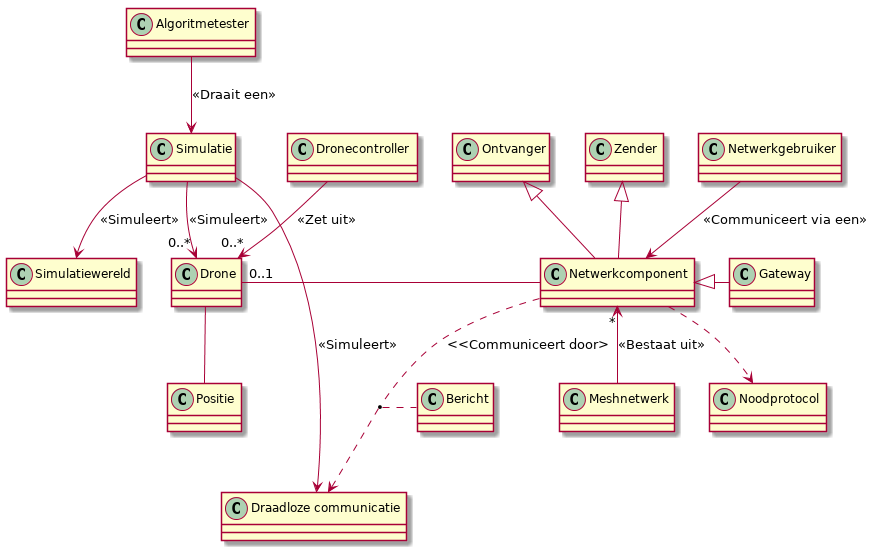
\includegraphics[width=\textwidth]{UML/out/DomeinModel/DomeinModel/DomeinModel.png}\end{center}
	\caption{Domeinmodel.}
	\label{fig:toplogienetwerkuml}
\end{figure}

\section{Beschrijving domeinmodel}
\label{domeinmodel:beschrijving}

\begin{longtable}[c]{|l|l|}
	\hline
	\rowcolor[HTML]{9B9B9B} 
	Term & Beschrijving \\ \hline
	\endhead
	%
	Algoritmetester & Een actor die algoritmes wil testen in een simulatie. \\ \hline
	Bericht & Een netwerkcomponent communiceert met berichten. \\ \hline
	Draadloze communicatie & \begin{tabular}[c]{@{}l@{}}Berichten worden verstuurd door het gebruik van \\ draadloze communicatie.\end{tabular} \\ \hline
	Drone & \begin{tabular}[c]{@{}l@{}}Een drone wordt ontplooit door een dronecontroller. \\ Het beschikt altijd over een netwerkcomponent. \\ Een drone heeft een positie.\end{tabular} \\ \hline
	Dronecontroller & \begin{tabular}[c]{@{}l@{}}Een dronecontroller is de actor die fysieke drones \\ ontplooit.\end{tabular} \\ \hline
	Gateway & \begin{tabular}[c]{@{}l@{}}Een gateway is een netwerkcomponent die het\\ netwerk van buitenaf benaderbaar maakt.\end{tabular} \\ \hline
	Meshnetwerk & \begin{tabular}[c]{@{}l@{}}Een meshnetwerk is een netwerktype waarin punten \\ dynamisch met elkaar kunnen verbinden en meerdere\\ connecties tegelijk aan kunnen gaan.\end{tabular} \\ \hline
	Netwerkcomponent & \begin{tabular}[c]{@{}l@{}}Een netwerkcomponent kan aangesloten worden op \\ een drone.  Het gebruikt draadloze communicatie om\\ berichten te versturen. Het gebruikt een noodprotocol.\\ Een netwerkcomponent is zowel een zender als een\\ ontvanger.\end{tabular} \\ \hline
	Netwerkgebruiker & \begin{tabular}[c]{@{}l@{}}Een netwerkgebruiker is een actor die wil communiceren\\ via het netwerk.\end{tabular} \\ \hline
	Noodprotocol & \begin{tabular}[c]{@{}l@{}}Een noodprotocol is een verzameling acties die ondernomen\\ worden zodra een component geen verbinding meer heeft.\end{tabular} \\ \hline
	Ontvanger & \begin{tabular}[c]{@{}l@{}}Een ontvanger is een rol binnen het netwerk voor het \\ ontvangen van berichten.\end{tabular} \\ \hline
	Positie & Een positie is een drie dimensionale plek in een ruimte.\\ \hline
	Simulatie & \begin{tabular}[c]{@{}l@{}}Een simulatie wordt gebruik om de wereld na te bootsen.\\ Een simulatie simuleert een wereld, drones en draadloze\\  communicatie.\end{tabular} \\ \hline
	Simulatiewereld & \begin{tabular}[c]{@{}l@{}}Een simulatie wereld  is een virtuele representatie van de\\ echte wereld.\end{tabular} \\ \hline
	Zender & \begin{tabular}[c]{@{}l@{}}Een zender is een rol binnen het netwerk voor het zenden\\van berichten.\end{tabular} \\ \hline
	\caption{Domeinmodel.}
	\label{tab:domeinmodel}\\
\end{longtable}

\chapter{Usecase omschrijvingen}
\label{Usecase}

\section[Simuleren dronenetwerk]{Usecase: Simuleren dronenetwerk}
\label{Usecase:simulatiedronenetwerk}
\subsection{Fully-dressed usecase description}

\begin{table}[H]
	\centering
	\begin{tabular}{|l|}
		\hline
		Usecase: Simuleren dronenetwerk. 				                                                                             \\ \hline
		Doel: De actor wil een dronenetwerk simuleren om algoritmes te testen zonder fysieke drones.                                    \\ \hline
		\begin{tabular}[c]{@{}l@{}}Beschrijving van de usecase:  De usecase start een simulatie op waarin een instelbaar aantal\\
								 drones gesimuleerd worden welke onderling kunnen communiceren via een gesimuleerde\\
								 draadloze communicatieweg. Hiermee creëren zij een meshnetwerk. \end{tabular} \\ \hline
		Stakeholder:  -                                                              \\ \hline
		Primary actor:  \nameref{inleiding:gebruikers:algoritmetester}.                                                               \\ \hline
		\begin{tabular}[c]{@{}l@{}} Preconditions: Er is in een configuratie aangegeven hoeveel router- en gatewaydrones\\gesimuleerd moeten worden. \end{tabular}                                        \\ \hline
		Postconditions: De simulatie van de drones en de communicatie is opgestart.                                                     \\ \hline
	\end{tabular}
\end{table}

\subsection{Basic Flow}
\begin{table}[H]
	\centering
	\begin{tabular}{|l|l|}
		\hline
		\rowcolor[HTML]{C0C0C0} 
		Actor actie  & System responsibility   \\ \hline
		  1. Past simulatie parameters aan.&  \\ \hline
		  2. Start de simulatie.		   &                     \\ \hline
		& 3. Toont de simulatie.                     \\ \hline
	\end{tabular}
\end{table}


\label{Usecase:simulatiedronenetwerk:fully-dressed}
\subsection{System Sequence Diagram}
\label{Usecase:simulatiedronenetwerk:systemsequence}
\begin{figure}[H]
	\begin{center}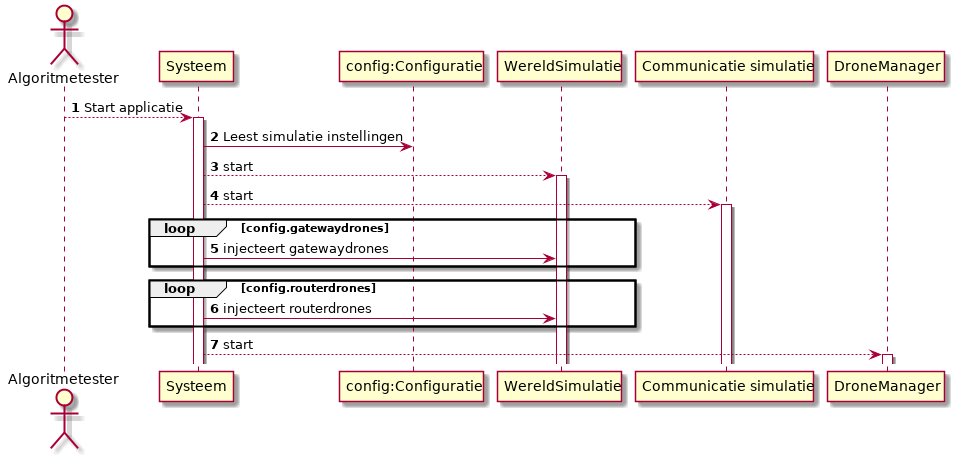
\includegraphics[height=.2\textheight]{UML/out/usecase/sequence/SimulerenDronenetwerk/SimulerenDronenetwerk.png}\end{center}
	\caption{System sequence diagram opstarten simulatie.}
	\label{fig:simulatiedronenetwerk:systemsequence}
\end{figure}


\section[Simuleren drone]{Usecase: Simuleren drone}
\label{Usecase:simulatiedrone}
\subsection{Fully-dressed usecase description}

\begin{table}[H]
	\centering
	\begin{tabular}{|l|}
		\hline
		Usecase: Simuleren drone.                                                                            \\ \hline
		Doel: Het creëren van een virtuele representatie van een drone.                                                                \\ \hline
		\begin{tabular}[c]{@{}l@{}}Beschrijving van de usecase: In de simulatie wil een actor een drone simuleren.\\
									Door het uitvoeren van deze usecase wordt er een drone in de simulatie geladen. \\ \end{tabular} \\ \hline
		Stakeholder: \nameref{Usecase:simulatiedronenetwerk}.                                                          \\ \hline						
		Primary actor:  \nameref{inleiding:gebruikers:algoritmetester}.                                                                                \\ \hline
		Preconditions: Er is een simulatiewereld aanwezig.                                                                         \\ \hline
		Postconditions: Een drone is ingeladen in de simulatiewereld.                                                     \\ \hline
	\end{tabular}
\end{table}

\subsection{Basic Flow }

\begin{table}[H]
	\centering
	\begin{tabular}{|l|l|}
		\hline
		\rowcolor[HTML]{C0C0C0} 
		Actor action  & System responsibility   \\ \hline
		1. Verzoekt een nieuwe drone.	& 2.  Toont een nieuwe drone in de simulatie              \\ \hline

	\end{tabular}
\end{table}


\label{Usecase:simulatiedrone:fully-dressed}
\subsection{System Sequence Diagram}
\label{Usecase:simulatiedrone:systemsequence}

\begin{figure}[H]
	\begin{center}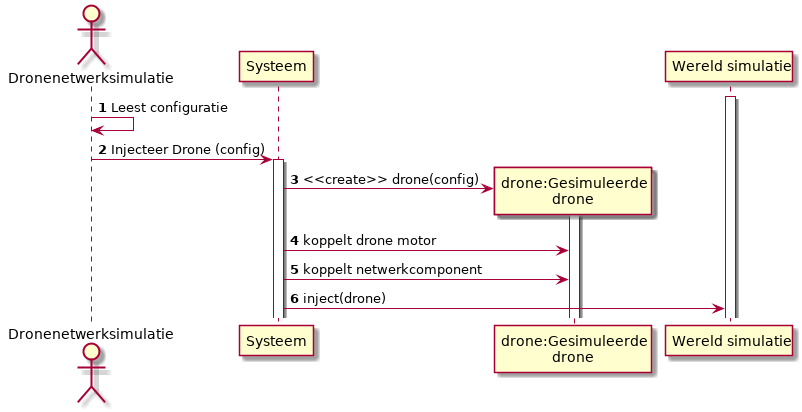
\includegraphics[height=.2\textheight]{UML/out/usecase/sequence/SimulerenDrone/SimulerenDrone.png}\end{center}
	\caption{System sequence diagram opstarten drone simulatie.}
	\label{fig:simulatiedrone:systemsequence}
\end{figure}

\hypertarget{draadlozecom}{
\section[Simuleren draadloze communicatie]{Usecase: Simuleren draadloze communicatie}}
\label{Usecase:simmulatiecommuicatie}
\subsection{Fully-dressed usecase description}

\begin{table}[H]
	\centering
	\begin{tabular}{|l|}
		\hline
		Usecase: Simuleren draadloze communicatie.                                                                            \\ \hline
		Doel: Het nabootsen van draadloze communicatie in een simulator.                               \\ \hline
		\begin{tabular}[c]{@{}l@{}}Beschrijving van de usecase: In de simulatie wil een actor gebruik maken van\\
								draadloze communicatie. Om dit realistisch na te bootsen loopt elk bericht langs\\
								de draadloos simulator die bepaalt wat er met het bericht gebeurt.\\ \end{tabular} \\ \hline
		Stakeholder: \nameref{Usecase:simulatiedronenetwerk}.                                                          \\ \hline						
		Primary actor:  \nameref{inleiding:gebruikers:algoritmetester}.                                                                                \\ \hline
		Preconditions:    -                                                                       \\ \hline
		\begin{tabular}[c]{@{}l@{}}Postconditions: Er is een simulator aanwezig die \nameref{Usecase:communicerendata} mogelijk\\maakt voor gesimuleerde \nameref{inleiding:werkomgeving:nrf24}'s.  \\ \end{tabular}   \\ \hline
	\end{tabular}
\end{table}

\subsection{Basic Flow}

\begin{table}[H]
	\centering
	\begin{tabular}{|l|l|}
		\hline
		\rowcolor[HTML]{C0C0C0} 
		Actor action  & System responsibility   \\ \hline
		\begin{tabular}[c]{@{}l@{}}1. Start draadloze communicatie applicatie.{}\end{tabular}\begin{tabular}[c]{@{}l@{}} {}\end{tabular}
		& 2. Start draadloze communicatie simulator.                  \\ \hline
		
	\end{tabular}
\end{table}

%\subsection{Alternative Flows}
%
%\begin{table}[H]
%	\centering
%	\begin{tabular}{|l|l|}
%		\hline
%		\rowcolor[HTML]{C0C0C0} 
%		Actor action  & System responsibility   \\ \hline
%		\begin{tabular}[c]{@{}l@{}}1. Start applicatie zonder\\ parameters.{}\end{tabular}&\begin{tabular}[c]{@{}l@{}}2. Start de communicatie simulatie met\\ de standaard waarde voor de maximale\\ communicatie afstand. {}\end{tabular}\\ \hline
%	\end{tabular}
%\end{table}

\label{Usecase:simmulatiecommuicatie:fully-dressed}
\subsection{System Sequence Diagram }
\label{Usecase:simmulatiecommuicatie:systemsequence}

\begin{figure}[H]
	\begin{center}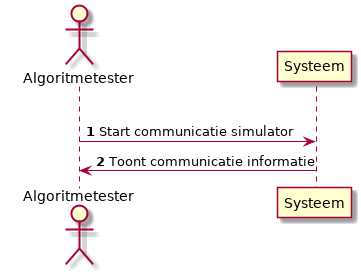
\includegraphics[height=.2\textheight]{UML/out/usecase/sequence/Simulerendraadlozecommunicatie/Simulerendraadlozecommunicatie.png}\end{center}
	\caption{System sequence diagram opstarten draadloze communicatie simulatie.}
	\label{fig:simmulatiecommuicatie:systemsequence}
\end{figure}

\section[Communiceren data]{Usecase: Communiceren data}
\label{Usecase:communicerendata}
\subsection{Fully-dressed usecase description}
\label{Usecase:communicerendata:fully-dressed}
\begin{table}[H]
	\centering
	\begin{tabular}{|l|}
		\hline
		Usecase: Communiceren data.					                                                                              \\ \hline
		Purpose: Deze usecase wordt gebruiken om data uit te wisselen tussen componenten                                             \\ \hline
		\begin{tabular}[c]{@{}l@{}}Beschrijving van de usecase: In het netwerk zullen componenten met elkaar willen \\communiceren. Deze usecase zal de data proberen te versturen. \\ \end{tabular} \\ \hline
		Stakeholder: \nameref{Usecase:simmulatiecommuicatie}, \nameref{Usecase:opbouwenmeshnetwerk}.                                                          \\ \hline						
		Primary actor:  \nameref{inleiding:gebruikers:netwerkgebruiker}, \nameref{inleiding:gebruikers:algoritmetester}, \nameref{inleiding:gebruikers:dronecontroller}                 \\ \hline
		 \begin{tabular}[c]{@{}l@{}}Preconditions: Communicatiemiddel van de zender is opgestart, de te versturen data is bekend,\\ en het adres van de ontvanger is bekend.{}\end{tabular}\\ \hline
		Postconditions: Er is data verstuurd van een component naar een andere component.                                           \\ \hline
	\end{tabular}
\end{table}

\subsection{Basic Flow }

\begin{table}[H]
	\centering
	\begin{tabular}{|l|l|}
		\hline
		\rowcolor[HTML]{C0C0C0} 
		Actor action  & System responsibility   \\ \hline
		1. Geeft bericht om te verzenden. & 2. Geeft succes aan van het versturen  \\ \hline
	\end{tabular}
\end{table}


\subsection{System Sequence Diagram }
\label{Usecase:communicerendata:systemsequence}

\begin{figure}[H]
	\begin{center}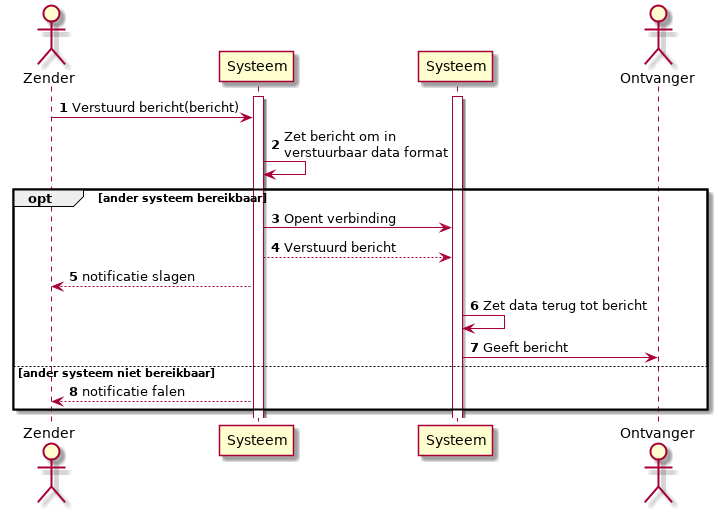
\includegraphics[height=.2\textheight]{UML/out/usecase/sequence/VersturenBericht/VersturenBericht.png}\end{center}
	\caption{System sequence diagram opstarten draadloze communicatie simulatie.}
	\label{fig:communicerendata:systemsequence}
\end{figure}

\section[Opbouwen meshnetwerk]{Usecase: Opbouwen meshnetwerk}
\label{Usecase:opbouwenmeshnetwerk}
\subsection{Fully-dressed usecase description}

\begin{table}[H]
	\centering
	\begin{tabular}{|l|}
		\hline
		Usecase: Opbouwen meshnetwerk.				                                                                              \\ \hline
		\begin{tabular}[c]{@{}l@{}} Doel: Het uitvoeren van de usecase zal een netwerk opzetten van onderling\\ verbonden netwerkcomponenten.\end{tabular}  \\ \hline
		\begin{tabular}[c]{@{}l@{}}Beschrijving van de usecase:  Na het uitvoeren van de usecase moeten alle\\ meshnetwerkcomponenten een verbinding hebben met de netwerkcomponenten die\\ binnen hun bereik zijn. De componenten staan klaar om berichten door te sturen \\naar elkaar of naar een gateway voor externe adressen.\end{tabular} \\ \hline
		Stakeholder: \nameref{Usecase:ontplooien}.                                                          \\ \hline						
		Primary actor:  \nameref{inleiding:gebruikers:algoritmetester}, \nameref{inleiding:gebruikers:dronecontroller}.                                                          \\ \hline
		\begin{tabular}[c]{@{}l@{}} Preconditions: Componenten zijn binnen bereik van elkaar, er is minstens één \\gateway aanwezig.\end{tabular}		                      \\ \hline
		Postconditions: Er is een onderling verbonden netwerk opgebouwd.                                                                       \\ \hline
	\end{tabular}
\end{table}

\subsection{Basic Flow }


\begin{table}[H]
	\centering
	\begin{tabular}{|l|l|}
		\hline
		\rowcolor[HTML]{C0C0C0} 
		Actor action  & System responsibility   \\ \hline
		1. Start netwerkcomponent. & \begin{tabular}[c]{@{}l@{}} 2. Geeft feedback over verbinding met een gateway\\ en/of andere punten. {}\end{tabular}	\\ \hline
	\end{tabular}
\end{table}

%\subsection{Alternative Flows}
%\begin{table}[H]
%	\centering
%	\begin{tabular}{|l|l|}
%		\hline
%		\rowcolor[HTML]{C0C0C0} 
%		Actor action  & System responsibility   \\ \hline
%		& 3. Componenten maken geen directe of indirecte verbinding met een gateway.\\ \hline
%		& 4. Componenten starten \nameref{Usecase:noodprotocol}.      \\ \hline
%	\end{tabular}
%\end{table}

\label{Usecase:opbouwenmeshnetwerk:fully-dressed}
\subsection{System Sequence Diagram }
\label{Usecase:opbouwenmeshnetwerk:systemsequence}

\begin{figure}[H]
	\begin{center}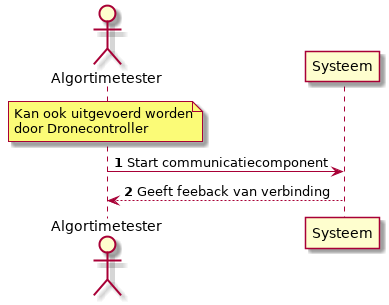
\includegraphics[height=.2\textheight]{UML/out/usecase/sequence/meshnetwerk/meshnetwerk.png}\end{center}
	\caption{System sequence diagram opzetten meshnetwerk.}
	\label{fig:opbouwenmeshnetwerk:systemsequence}
\end{figure}


\hypertarget{noodprotocol}{\section[Uitvoeren noodprotocol bij geen verbinding]{Usecase: Uitvoeren noodprotocol bij geen verbinding}}
\label{Usecase:noodprotocol}
\subsection{Fully-dressed usecase description}
\label{Usecase:noodprotocol:fully-dressed}

\begin{table}[H]
	\centering
	\begin{tabular}{|l|}
		\hline
		Usecase: Uitvoeren noodprotocol bij geen verbinding.                                                                              \\ \hline
		\begin{tabular}[c]{@{}l@{}}Doel: Door het uitvoeren van een noodprotocol zijn één of meerdere drones in staat\\de verbinding te herstellen met een gateway. Hiervoor kan het gebruik maken van\\ \nameref{Usecase:aansturendrone}.{}\end{tabular}\\ \hline
		\begin{tabular}[c]{@{}l@{}}Beschrijving van de usecase: Deze usecase is de uiterste stap die een netwerkcomponent \\onderneemt bij het verlies van een verbinding.\end{tabular} \\ \hline
		Stakeholder: \nameref{Usecase:opbouwenmeshnetwerk}.                                                          \\ \hline						
		Primary actor:  \nameref{inleiding:gebruikers:algoritmetester}.                                                                                \\ \hline
		Preconditions: 	Elke drone heeft een locatie van een gateway.		                                                                          \\ \hline
		\begin{tabular}[c]{@{}l@{}} Postconditions: 1: Drone(s) is/zijn verplaatst naar een positie in verbinding met een gateway.\\2: Drone(s) zijn verplaatst naar de positie van de gateway.\end{tabular} \\ \hline
	\end{tabular}
\end{table}

\subsection{Basic Flow }


\begin{table}[H]
	\centering
	\begin{tabular}{|l|l|}
		\hline
		\rowcolor[HTML]{C0C0C0} 
		Actor action  & System responsibility   \\ \hline
		1. Start noodprotocol. &  2. Drones herpositioneren zich.\\ \hline
	\end{tabular}
\end{table}

\subsection{Alternative Flows}


\begin{table}[H]
	\centering
	\begin{tabular}{|l|l|}
		\hline
		\rowcolor[HTML]{C0C0C0} 
		Actor action  & System responsibility   \\ \hline
	    &  2. Drone positioneert zich op nieuwe locatie.     \\ \hline
	\end{tabular}
\end{table}

\begin{table}[H]
	\centering
	\begin{tabular}{|l|l|}
		\hline
		\rowcolor[HTML]{C0C0C0} 
		Actor action  & System responsibility   \\ \hline
		&  3. Drone(s) keren terug naar de positie van de gateway. \\ \hline
	\end{tabular}
\end{table}

\subsection{System Sequence Diagram }
\label{Usecase:noodprotocol:systemsequence}

\begin{figure}[H]
	\begin{center}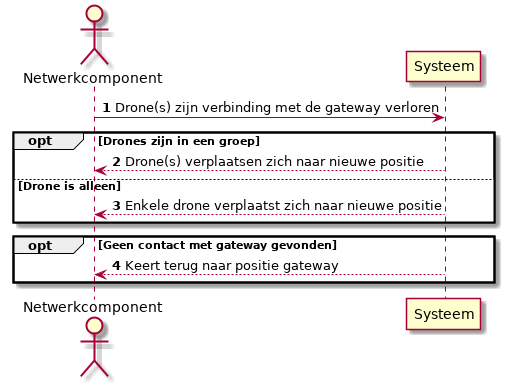
\includegraphics[height=.3\textheight]{UML/out/usecase/sequence/noodprotocol/noodprotocol.png}\end{center}
	\caption{System sequence diagram noodprotocol.}
	\label{fig:noodprotocol:systemsequence}
\end{figure}


\section[Ontplooien dronenetwerk]{Usecase: Ontplooien dronenetwerk}
\label{Usecase:ontplooien}
\subsection{Fully-dressed usecase description}
\label{Usecase:ontplooien:fully-dressed}

\begin{table}[H]
	\centering
	\begin{tabular}{|l|}
		\hline
		Usecase: Ontplooien dronenetwerk.                                                                             \\ \hline
		\begin{tabular}[c]{@{}l@{}}Doel: Het doel van deze usecase is het ontplooien van een dronenetwerk, met\\een posities zal worden aangegeven waar naartoe te verplaatsen, ze moeten\\ zelfstandig een netwerk opzetten.{}\end{tabular}   \\ \hline
		\begin{tabular}[c]{@{}l@{}}Beschrijving van de usecase: Deze usecase zal alle drones aansturen om naar\\ een vooraf bepaalde posities te vliegen. De drones zullen een meshnetwerk\\ opbouwen waarover gecommuniceerd kan worden. \\ \end{tabular} \\ \hline
				Stakeholder: \nameref{Usecase:simulatiedronenetwerk}.                                                          \\ \hline						
		Primary actor:  \nameref{inleiding:gebruikers:dronecontroller}, \nameref{inleiding:gebruikers:algoritmetester}  \\ \hline
		\begin{tabular}[c]{@{}l@{}}Preconditions: Drones zijn voorzien van netwerkcomponenten en kunnen zich\\verplaatsen. Voor elke drone is een doel bekend.\end{tabular} \\ \hline
		\begin{tabular}[c]{@{}l@{}}Postconditions: Drones zijn verplaatst naar ingestelde positie en hebben\\een onderling netwerk opgebouwd.{}\end{tabular} \\ \hline
	\end{tabular}
\end{table}

\subsection{Basic Flow }


\begin{table}[H]
	\centering
	\begin{tabular}{|l|l|}
		\hline
		\rowcolor[HTML]{C0C0C0} 
		Actor action  & System responsibility   \\ \hline
		1. Start alle drones op. 		& \\ \hline
		2. Geeft posities door voor de drones.  & 3. Stuurt elke individuele drone aan naar positie.    \\ \hline
												& 4. Meshcomponenten bouwen netwerk op.                 \\ \hline
	\end{tabular}
\end{table}

\subsection{Alternative Flows}


\begin{table}[H]
	\centering
	\begin{tabular}{|l|l|}
		\hline
		\rowcolor[HTML]{C0C0C0} 
		Actor action  & System responsibility   \\ \hline
		& 3. De drones die bereikbaar zijn in het netwerk verplaatsen zich.      	    \\ \hline
	\end{tabular}
\end{table}

\subsection{System Sequence Diagram }
\label{Usecase:ontplooien:systemsequence}


\begin{figure}[H]
	\begin{center}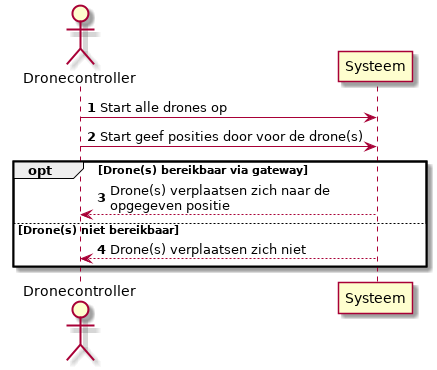
\includegraphics[height=.3\textheight]{UML/out/usecase/sequence/ontplooien/ontplooien.png}\end{center}
	\caption{System sequence diagram noodprotocol.}
	\label{fig:ontplooien:systemsequence}
\end{figure}


\section[Verzoeken droneverplaatsing]{Usecase: Verzoeken droneverplaatsing}
\label{Usecase:verzoekverplaatsing}
\subsection{Fully-dressed usecase description}
\label{Usecase:verzoekverplaatsing:fully-dressed}
\begin{table}[H]
	\centering
	\begin{tabular}{|l|}
		\hline
		Usecase: Verzoeken droneverplaatsing.                                                                              \\ \hline
		Doel: Deze usecase dient voor het verzoeken tot een verplaatsing van een drone.                                    \\ \hline
		\begin{tabular}[c]{@{}l@{}}Beschrijving usecase: Door deze usecase te gebruiken kan een individuele\\drone verzocht worden zich te verplaatsen.  {}\end{tabular} \\ \hline
		Stakeholder: \nameref{Usecase:ontplooien}, \nameref{Usecase:simulatiedronenetwerk}.                                                          \\ \hline						
		Primary actor:  \nameref{inleiding:gebruikers:dronecontroller}, \nameref{inleiding:gebruikers:algoritmetester}. \\ \hline
		Preconditions: Communicatieweg beschikbaar tot aan drone.\\ \hline
		Postconditions: Drone gaat zich verplaatsen naar verzoeklocatie.            \\ \hline
	\end{tabular}
\end{table}

\subsection{Basic Flow }


\begin{table}[H]
	\centering
	\begin{tabular}{|l|l|}
		\hline
		\rowcolor[HTML]{C0C0C0} 
		Actor action  & System responsibility   \\ \hline
		1. Verstuurt verzoek voor verplaatsing.  & 2. Drone verplaatst zich naar positie. \\ \hline
												 	\end{tabular}
\end{table}

\subsection{Alternative Flows}


\begin{table}[H]
	\centering
	\begin{tabular}{|l|l|}
		\hline
		\rowcolor[HTML]{C0C0C0} 
		Actor action  & System responsibility   \\ \hline
	    & 2. Drone blijft staan. \\ \hline
	\end{tabular}
\end{table}


\subsection{System Sequence Diagram }
\label{Usecase:verzoekverplaatsing:systemsequence}

\begin{figure}[H]
	\begin{center}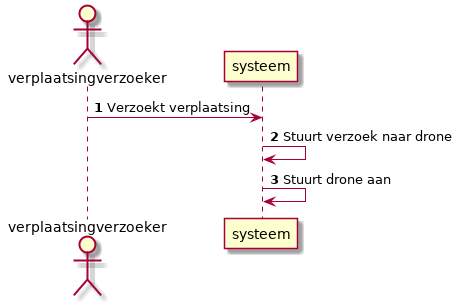
\includegraphics[height=.3\textheight]{UML/out/usecase/sequence/verzoekendroneverplaatsing/verzoekendroneverplaatsing.png}\end{center}
	\caption{System sequence verzoeken verplaatsing.}
	\label{fig:verzoekverplaatsing:systemsequence}
\end{figure}


\section[Aansturen drone]{Usecase: Aansturen drone}
\label{Usecase:aansturendrone}
\subsection{Fully-dressed usecase description}
\label{Usecase:aansturendrone:fully-dressed}
\begin{table}[H]
	\centering
	\begin{tabular}{|l|}
		\hline
		Usecase: Aansturen drone.                                                                             \\ \hline
		Purpose: Het aansturen van een drone wordt gebruikt om een drone te verplaatsen.                                                                               \\ \hline
		\begin{tabular}[c]{@{}l@{}}Beschrijving van de usecase: Elke drone kan aangestuurd worden om zich te verplaatsen.\\Dit wordt altijd uitgevoerd vanaf het aangesloten netwerkcomponent. Daarom moet er\\vanuit een extern punt altijd een verzoek gestuurd worden voor een verplaatsing of vanaf\\de aangesloten module zelf komen. {}\end{tabular} \\ \hline
		\begin{tabular}[c]{@{}l@{}} Stakeholder: \nameref{Usecase:verzoekverplaatsing}, \nameref{Usecase:noodprotocol},\\ \nameref{Usecase:simulatiedrone}.{}\end{tabular}             \\ \hline						
		Primary actor: \nameref{inleiding:gebruikers:dronecontroller}, \nameref{inleiding:gebruikers:algoritmetester}.                                        \\ \hline
		Preconditions: Drone is in staat zich te verplaatsen.                                                                         \\ \hline
		Postconditions: Drone heeft zich verplaatst naar de verzochte positie.                                                                   \\ \hline
	\end{tabular}
\end{table}

\subsection{Basic Flow }


\begin{table}[H]
	\centering
	\begin{tabular}{|l|l|}
		\hline
		\rowcolor[HTML]{C0C0C0} 
		Actor action  & System responsibility   \\ \hline
		1. Stuurt doellocatie. & 2. Verplaatst zich naar locatie. \\ \hline
	\end{tabular}
\end{table}

\subsection{Alternative Flows}


\begin{table}[H]
	\centering
	\begin{tabular}{|l|l|}
		\hline
		\rowcolor[HTML]{C0C0C0} 
		Actor action  & System responsibility   \\ \hline
				      & 2. Blijft op huidige locatie.                        \\ \hline
	\end{tabular}
\end{table}


\subsection{System Sequence Diagram }
\label{Usecase:aansturendrone:systemsequence}


\begin{figure}[H]
	\begin{center}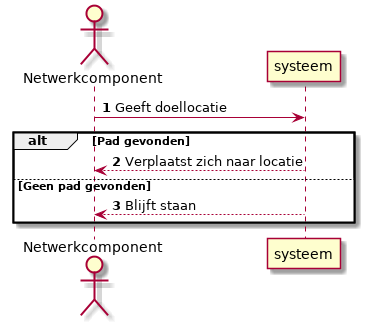
\includegraphics[height=.25\textheight]{UML/out/usecase/sequence/aansturendrone/aansturendrone.png}\end{center}
	\caption{System sequence aansturen drone.}
	\label{fig:aansturendrone:systemsequence}
\end{figure}


\chapter{Functionele requirements }
Voor dit project zijn er requirements opgesteld. Deze requirements zijn opgesteld a.d.h.v. de MoSCoW methode, hiervoor is gekozen om de requirements
te prioriteren. De Must requirements moeten voor het einde van het project gerealiseerd worden. De overige requirements hebben een lagere prioriteit en
hieraan wordt pas gewerkt als alle Must requirements afgehandeld zijn. Onder de tabel is per requirement een toelichting te vinden.
\begin{longtable}{|l|l|l|l|}
	\hline
	\rowcolor[HTML]{C0C0C0} 
	Naam & Beschrijving & MoSCoW\\ \hline
	%\endfirsthead
	%
	\endhead
	\hyperlink{SIMULATIE1}{SIMULATIE1}			&\begin{tabular}[c]{@{}l@{}}Simulatie representeert een wereld.	\end{tabular} 							 &M \\ \hline
	\hyperlink{SIMULATIE2}{SIMULATIE2}			&\begin{tabular}[c]{@{}l@{}}Simulatie simuleert en visualiseert een abstracte drone.\end{tabular}        &M \\ \hline
	\hyperlink{SIMULATIE3}{SIMULATIE3}			&\begin{tabular}[c]{@{}l@{}}Simulatie simuleert de beweging van een drone.\end{tabular}       			 &M \\ \hline
	\hyperlink{SIMULATIE4}{SIMULATIE4}			&\begin{tabular}[c]{@{}l@{}}Simulatie simuleert tot 100 drones tegelijk.\end{tabular}        			 &S \\ \hline	
	\hyperlink{SIMULATIE5}{SIMULATIE5}			&\begin{tabular}[c]{@{}l@{}}Simulatie simuleert draadloze communicatie.\end{tabular}        			 &M \\ \hline	
	\hyperlink{SIMULATIE6}{SIMULATIE6}			&\begin{tabular}[c]{@{}l@{}}Simulatie simuleert een Raspberry Pi. \end{tabular}        						 &S \\ \hline	
	\hyperlink{SIMULATIE7}{SIMULATIE7}			&\begin{tabular}[c]{@{}l@{}}Een gesimuleerde Raspberry Pi houdt zich aan de\\snelheidslimieten van een Raspberry Pi model 2B+. \end{tabular}        						 &W \\ \hline	
	\hyperlink{SIMULATIE8}{SIMULATIE8}			&\begin{tabular}[c]{@{}l@{}}Simulatie kan met een configuratiebestand gestart worden. \end{tabular}     &S \\ \hline	
	\hyperlink{DRONE1}{DRONE1}		&\begin{tabular}[c]{@{}l@{}}Drone kan zich verplaatsen naar een positie. \end{tabular}        			 &M \\ \hline	
	\hyperlink{DRONE2}{DRONE2}		&\begin{tabular}[c]{@{}l@{}}Drone kan een route naar positie berekenen.  \end{tabular}        			 &S \\ \hline	
	\hyperlink{DRONE3}{DRONE3}		&\begin{tabular}[c]{@{}l@{}}Drone kan een locatie aanbieden.  \end{tabular}        						 &M \\ \hline	
	\hyperlink{DRONE4}{DRONE4}		&\begin{tabular}[c]{@{}l@{}}Drone is voorzien van een netwerkcomponent.  \end{tabular}       &M \\ \hline	
	\hyperlink{NETWERK1}{NETWERK1}	&\begin{tabular}[c]{@{}l@{}}Netwerk kan zelfstandig een meshnetwerk opbouwen. \end{tabular}    			 &M \\ \hline	
	\hyperlink{NETWERK2}{NETWERK2}	&\begin{tabular}[c]{@{}l@{}}Netwerk heeft altijd minstens 1 gateway. 	\end{tabular}			 &M \\ \hline	
	\hyperlink{NETWERK3}{NETWERK3}	&\begin{tabular}[c]{@{}l@{}}Netwerk kan drones aansturen.						 \end{tabular}			 &M \\ \hline	
	\hyperlink{NETWERK4}{NETWERK4}	&\begin{tabular}[c]{@{}l@{}}Netwerk biedt een externe interface voor aansturing aan. \end{tabular}		 &S \\ \hline	
	\hyperlink{NETWERK5}{NETWERK5}	&\begin{tabular}[c]{@{}l@{}}Netwerk kan onderling data communiceren.	 \end{tabular}					 &M \\ \hline	
	\hyperlink{NETWERK6}{NETWERK6}	&\begin{tabular}[c]{@{}l@{}}Netwerk kan zichzelf herstellen. \end{tabular}			 					 &M \\ \hline	
	\hyperlink{NETWERK7}{NETWERK7}	&\begin{tabular}[c]{@{}l@{}}Meerdere gateways kunnen tegelijk aanwezig zijn in het\\ netwerk. \end{tabular}			 					 &C \\ \hline	
	\hyperlink{ALGORITME1}{ALGORITME1}		&\begin{tabular}[c]{@{}l@{}}Algoritmetester kan drones verdelen. \end{tabular}		 					 &M \\ \hline	
	\hyperlink{ALGORITME2}{ALGORITME2}		&\begin{tabular}[c]{@{}l@{}}Algoritmetester kan een casus met een verdeling starten. \end{tabular}		 					 &C \\ \hline	
	\caption{Functionele requirements.}
	\label{tab:criteria}
\end{longtable}

\section{Toelichting functionele requirements}

\subsection{Simulatie}
Onderstaand worden alle functionele requirements van de simulatie toegelicht.
\paragraph{SIMULATIE1: Simulatie representeert een wereld}
\hypertarget{SIMULATIE1}{}

De simulatiecomponent moet een echte wereld nabootsen, er hoeven nog geen objecten in aanwezig te zijn.
Een simulatiewereld bestaat uit een ruimte en maakt gebruiken van tijd. 
De simulatiewereld moet in staat zijn krachten afkomstig van zwaartekracht, botsingen en wrijving te verwerken. 

\paragraph{SIMULATIE2: Simulatie simuleert en visualiseert een abstracte drone.}
\hypertarget{SIMULATIE2}{}

De simulatie moet een abstracte versie van een drone representeren hierbij maakt de vorm niet uit zolang er maar een verschil te zien is tussen het type drone.

\paragraph{SIMULATIE3: Simulatie simuleert de beweging van een drone.}
\hypertarget{SIMULATIE3}{}

De drone moet bewegen in de simulatie, het is belangrijk dat deze beweging visueel zichtbaar is voor analyse van het verplaatsingsgedrag.

\paragraph{SIMULATIE4: Simulatie simuleert tot 100 drones tegelijk.}
\hypertarget{SIMULATIE4}{}

Om met meerdere drones te kunnen testen moet de simulatie tot aan honderd drones tegelijk kunnen simuleren dit hoeft niet visueel te gebeuren om de grafische kaart te ontlasten.

\paragraph{SIMULATIE5: Simulatie simuleert draadloze communicatie.}
\hypertarget{SIMULATIE5}{}

Omdat er een simulatie van een meshnetwerk gerealisseerd wordt moet er een component aanwezig zijn die zorgt dat de draadloze communicatie volgens de juiste regels verloopt.

\paragraph{SIMULATIE6: Simulatie simuleert een Raspberry Pi.}
\hypertarget{SIMULATIE6}{}

In het project wordt gebruik gemaakt van het Raspberry Pi model 2B+ deze moet virtueel gerepresenteerd worden door de simulatie.

\paragraph{SIMULATIE7: Een gesimuleerde Raspberry Pi houdt zich aan de snelheidslimieten van een Raspberry Pi model 2B+.}
\hypertarget{SIMULATIE7}{}

De gesimuleerde Raspberry Pi zal zich niet houden aan de clock snelheid van een echte Raspberry Pi model 2B+.

\paragraph{SIMULATIE8: Simulatie kan met een configuratiebestand gestart worden.}
\hypertarget{SIMULATIE8}{}

Om het starten van simulaties gemakkelijk te maken voor de algoritmetester moet het mogelijk zijn simulaties via een configuratie op te starten.


\subsection{Drone}
Onderstaand worden alle functionele requirements van de drone toegelicht.
\paragraph{DRONE1: Drone kan zich verplaatsen naar een positie}
\hypertarget{DRONE1}{}

Het netwerk rekent op de mogelijkheid van een drone om zich te kunnen verplaatsen om zo het herstellend vermogen te vergroten.

\paragraph{DRONE2: Drone kan een route naar positie berekenen}
\hypertarget{DRONE2}{}

Een drone moet op basis van een ontvangen doel zich kunnen verplaatsen naar een positie. Om deze verplaatsingen uit te kunnen voeren maakt hij gebruik van een zelf berekende route.

\paragraph{DRONE3: Drone kan een locatie aanbieden}
\hypertarget{DRONE3}{}

Een netwerkmodule is zelf niet voorzien van een component voor het ophalen van een locatie daarvoor maakt hij gebruik van de drone. Daarom moet een drone in staat zijn om zijn locatie door te geven.

\paragraph{DRONE4: Drone is voorzien van een meshnetwerkcomponent}
\hypertarget{DRONE4}{}

Een drone moet worden voorzien van een meshnetwerkcomponent om zo alle drones wanneer mogelijk met elkaar te kunnen laten communiceren.

\subsection{Netwerk}
Onderstaand worden alle functionele requirements van het netwerk toegelicht.

\paragraph{NETWERK1: Netwerk kan zelfstandig een meshnetwerk opbouwen}
\hypertarget{NETWERK1}{}

De opzetter van het netwerk wil zich niet bezig hoeven houden met het onderling verbinden van de drones. De netwerkmodules moeten zelf een netwerk opzetten zonder tussenkomst van menselijke actoren.

\paragraph{NETWERK2: Netwerk biedt altijd minstens 1 gateway aan}
\hypertarget{NETWERK2}{}

Om het netwerk toegang te kunnen geven tot een extern punt moet er tenminste altijd een gateway aanwezig zijn in het netwerk.

\paragraph{NETWERK3: Netwerk kan drones aansturen}
\hypertarget{NETWERK3}{}

Het netwerk is zelf in staat drones aan te sturen wanneer er een verplaatsing vereist is, het netwerk kan deze beslissing zelfstandig maken.

\paragraph{NETWERK5: Netwerk kan onderling data communiceren}
\hypertarget{NETWERK5}{}

De essentie van het netwerk is natuurlijk de mogelijkheid om onderling data te kunnen communiceren. Dit wordt gebruikt voor het opzetten en onderhoud van het netwerk. Daarnaast kunnen gebruikers gebruik maken van het netwerk om data te communiceren.

\paragraph{NETWERK6: Netwerk kan zichzelf herstellen}
\hypertarget{NETWERK6}{}

Wanneer het netwerk zijn onderlinge verbinding verliest moet het deze zelf kunnen herstellen, dit gebeurt door een nieuwe route te creëren of door de drone(s) te herverdelen.

\paragraph{NETWERK7: Meerdere gateways kunnen tegelijk aanwezig zijn in het netwerk}
\hypertarget{NETWERK7}{}

Om de stabiliteit van het netwerk te vergroten moet het mogelijk zijn het netwerk te ontplooien met meerdere gateways. 


\subsection{Algoritme testapplicatie}
Onderstaand worden alle functionele requirements van de testapplicatie voor het algoritme toegelicht.
\paragraph{ALGORITME1: Algoritmetester kan drones verdelen.}
\hypertarget{ALGORITME1}{}
Een algoritmetester moet om zijn algoritme te kunnen testen drones kunnen verplaatsen, dit zal via een aangeboden interface gebeuren.
\paragraph{ALGORITME2: Algoritmetester kan een casus met een verdeling starten}
\hypertarget{ALGORITME2}{}
Een algoritmetester moet casus situaties kunnen testen deze casus zal aangeroepen worden via een API. 

\chapter{Non-functionele requirements}
\section{Performance efficiency}

\begin{longtable}{|l|l|l|}
	\hline
	\rowcolor[HTML]{C0C0C0} 
	Naam & Beschrijving \\ \hline
	%\endfirsthead
	%
	\endhead
	\hyperlink{PERF1}{PERF1}			&\begin{tabular}[c]{@{}l@{}}Simulatiesnelheid moet minimaal 50 procent van de realiteit hebben.	\end{tabular}\\ \hline
	%\hyperlink{PERF2}{PERF2}			&\begin{tabular}[c]{@{}l@{}}Een router moet `snel` een pad berekenen.\end{tabular}\\ \hline
	\hyperlink{PERF2}{PERF2}			&\begin{tabular}[c]{@{}l@{}}Een drone kan binnen 10 seconden zijn positie bepalen.\end{tabular}\\ \hline
	\caption{Non-functionele requirements performance.}
	\label{tab:nietfunctionelecriteria:performance}
\end{longtable}

\section{Security}

\begin{longtable}{|l|l|l|}
	\hline
	\rowcolor[HTML]{C0C0C0} 
	Naam & Beschrijving \\ \hline
	%\endfirsthead
	%
	\endhead
	\hyperlink{SEC1}{SEC1}			&\begin{tabular}[c]{@{}l@{}}Een drone mag alleen door een netwerkmodule aangestuurd worden.\end{tabular}\\ \hline
	\caption{Non-functionele requirements security.}
	\label{tab:nietfunctionelecriteria:security}
\end{longtable}

\section{Reliability}

\begin{longtable}{|l|l|l|}
	\hline
	\rowcolor[HTML]{C0C0C0} 
	Naam & Beschrijving \\ \hline
	%\endfirsthead
	%
	\endhead
	\hyperlink{REL1}{REL1}			&\begin{tabular}[c]{@{}l@{}}Het netwerk mag maximaal 5 procent van zijn berichten verliezen.	\end{tabular}\\ \hline
	\hyperlink{REL2}{REL2}			&\begin{tabular}[c]{@{}l@{}}Een router heeft altijd direct of indirect een verbinding met een gateway.	\end{tabular}\\ \hline
	\caption{Non-functionele requirements reliabilty.}
	\label{tab:nietfunctionelecriteria:reliabilty}
\end{longtable}

\section{Timeliness}

\begin{longtable}{|l|l|l|}
	\hline
	\rowcolor[HTML]{C0C0C0} 
	Naam & Beschrijving \\ \hline
	%\endfirsthead
	%
	\endhead
	\hyperlink{TIME1}{TIME1}			&\begin{tabular}[c]{@{}l@{}}Het netwerk moet binnen 30 seconden detecteren dat er\\ een verbinding verloren is.	\end{tabular}\\ \hline
	\hyperlink{TIME2}{TIME2}			&\begin{tabular}[c]{@{}l@{}}Het netwerk moet minus de tijd van het verplaatsen van de drones\\zich herstellen binnen 2 minuten.\end{tabular}\\ \hline
	\caption{Non-functionele requirements timeliness.}
	\label{tab:nietfunctionelecriteria:timeliness}
\end{longtable}

\section{Quality}

\begin{longtable}{|l|l|l|}
	\hline
	\rowcolor[HTML]{C0C0C0} 
	Naam & Beschrijving \\ \hline
	%\endfirsthead
	%
	\endhead
	\hyperlink{QUA1}{QUA1}			&\begin{tabular}[c]{@{}l@{}} Het netwerk moet een minimale snelheid van \SI{100}{\kilo\bit\per\second} ondersteunen. \end{tabular}\\ \hline
	\caption{Non-functionele requirements quality.}
	\label{tab:nietfunctionelecriteria:quality}
\end{longtable}

\section{Scalability}

\begin{longtable}{|l|l|l|}
	\hline
	\rowcolor[HTML]{C0C0C0} 
	Naam & Beschrijving \\ \hline
	%\endfirsthead
	%
	\endhead
	\hyperlink{SCALE1}{SCALE1}			&\begin{tabular}[c]{@{}l@{}} Een netwerkmodule past op elke drone die voldoet aan de gevraagde interface.	\end{tabular}\\ \hline
	\caption{Non-functionele requirements scalability.}
	\label{tab:nietfunctionelecriteria:scalability}
\end{longtable}

\chapter{Bewijslast gestelde requirements}
Om aan te tonen dat zowel functionele als niet functionele requirements zijn behaald wordt er gebruik gemaakt van verwijzingen. Dit gebeurt door het verwijzen naar een usecase maar ook door het verwijzen naar andere documenten, demonstraties of code in de onderstaande tabel.

\begin{longtable}[c]{|l|l|}
	\hline
	\rowcolor[HTML]{C0C0C0} 
	Requirement & Bewijs \\ \hline
	\endhead
	%
\hyperlink{SIMULATIE1}{SIMULATIE1}	& \begin{tabular}[c]{@{}l@{}} Er is onderzocht welke simulatiesoftware gebruikt moet worden om\\aan deze eis te voldoen. Dit is terug te lezen in bijlage \ref{sec:onderzoeksrapport-drone-meshnetwerk-simulatie}. De\\gekozen software is gazebo.	\end{tabular} \\ \hline
\hyperlink{SIMULATIE2}{SIMULATIE2}	& \begin{tabular}[c]{@{}l@{}} In het onderzoek van bijlage \ref{sec:onderzoeksrapport-drone-meshnetwerk-simulatie} is bepaald wat een abstracte drone\\inhoudt. Dit is gerealiseerd in de code van de class VirtualDrone  te\\vinden in \autoref{app:broncode}. De werking wordt toegelicht in bijlage \ref{sec:softwaredesigndocument}.  \end{tabular} \\ \hline
\hyperlink{SIMULATIE3}{SIMULATIE3}	& \begin{tabular}[c]{@{}l@{}} Dit is gerealiseerd in de code van de class DroneEngine  te\\vinden in \autoref{app:broncode}. De werking wordt toegelicht in bijlage \ref{sec:softwaredesigndocument}.	\end{tabular} \\ \hline
\hyperlink{SIMULATIE4}{SIMULATIE4}	& \begin{tabular}[c]{@{}l@{}} De simulatie kan met honderd drones tegelijk draaien, dit is te zien\\in bijlage \ref{sec:gateway-drone-en-99-routerdronesmp4}.\end{tabular}\\ \hline
\hyperlink{SIMULATIE5}{SIMULATIE5}	& \begin{tabular}[c]{@{}l@{}} In de demonstratie video's te vinden in bijlage \ref{sec:videos-simulatie-netwerkherstel-door-drone-verplaatsing} is te zien dat de\\drones met elkaar communiceren. Dit is gerealiseerd in de code van\\de folder drone\_meshnetwork\_simulation/src/ros/WirelessSimulation\\te vinden in \autoref{app:broncode}.	\end{tabular} \\ \hline
\hyperlink{SIMULATIE6}{SIMULATIE6}	& \begin{tabular}[c]{@{}l@{}}Dit is gerealiseerd in de code van de folder drone\_meshnetwork\_sim\\-ulation/src/gazebo/RaspberryPi te vinden in \autoref{app:broncode}. 	\end{tabular} \\ \hline
\hyperlink{SIMULATIE8}{SIMULATIE8}	& \begin{tabular}[c]{@{}l@{}} De simulatie kan geconfigureerd worden met factory.world bestand\\te vinden in \autoref{app:broncode}.	\end{tabular} \\ \hline
\hyperlink{DRONE1}{DRONE1}			& \begin{tabular}[c]{@{}l@{}}  Dit is gerealiseerd in de code van de class DroneEngine  te\\vinden in \autoref{app:broncode}. De werking wordt toegelicht in bijlage \ref{sec:softwaredesigndocument}.	\end{tabular} \\ \hline
\hyperlink{DRONE2}{DRONE2}			& \begin{tabular}[c]{@{}l@{}}  Dit is gerealiseerd in de code van de class DroneEngine  te\\vinden in \autoref{app:broncode}. De werking wordt toegelicht in bijlage \ref{sec:softwaredesigndocument}.	\end{tabular} \\ \hline
\hyperlink{DRONE3}{DRONE3}			& \begin{tabular}[c]{@{}l@{}}  Dit is gerealiseerd in de code van de class DroneEngine  te\\vinden in \autoref{app:broncode}. De werking wordt toegelicht in bijlage \ref{sec:softwaredesigndocument}.	\end{tabular} \\ \hline
\hyperlink{DRONE4}{DRONE4}			& \begin{tabular}[c]{@{}l@{}} In het onderzoek van bijlage \ref{sec:onderzoeksrapport-drone-meshnetwerk-simulatie} is bepaald wat een abstracte drone\\inhoudt. Dit is gerealiseerd in de code van de class VirtualDrone  te\\vinden in \autoref{app:broncode}. De werking wordt toegelicht in bijlage \ref{sec:softwaredesigndocument}.	\end{tabular} \\ \hline
\hyperlink{NETWERK1}{NETWERK1}		& \begin{tabular}[c]{@{}l@{}} In de demonstratie videos te vinden in bijlage \ref{sec:videos-simulatie-netwerkherstel-door-drone-verplaatsing}, \ref{sec:gateway-drone-en-99-routerdronesmp4} is te zien dat\\de netwerkmodules zelfstandig een netwerk opbouwen in een\\simulatie. De werking op de raspberry is te zien in bijlage \ref{sec:fysieke-router-en-dronemp4}	\end{tabular} \\ \hline
\hyperlink{NETWERK2}{NETWERK2}		& \begin{tabular}[c]{@{}l@{}} In het SDD  te vinden in bijlage \ref{sec:softwaredesigndocument} is vinden dat de routers altijd\\bezig zijn met zoeken naar een gateway.	\end{tabular} \\ \hline
\hyperlink{NETWERK3}{NETWERK3}		& \begin{tabular}[c]{@{}l@{}} In de bijlage \ref{sec:fysieke-router-en-dronemp4} is te zien dat er locatie via het netwerk naar een\\drone verstuurd wordt.	\end{tabular} \\ \hline
\hyperlink{NETWERK4}{NETWERK4}		& \begin{tabular}[c]{@{}l@{}} Dit is gerealiseerd in de code van de class InternetGateway  te\\vinden in \autoref{app:broncode}.	Werkend te zien in bijlage \ref{sec:fysieke-router-en-dronemp4}\end{tabular} \\ \hline
\hyperlink{NETWERK5}{NETWERK5}		& \begin{tabular}[c]{@{}l@{}} In de demonstratie video's te vinden in bijlage \ref{sec:videos-simulatie-netwerkherstel-door-drone-verplaatsing} is te zien dat de\\drones met elkaar communiceren. Dit is gerealiseerd in de code van\\de folder drone\_meshnetwork\_simulation/src/ros/WirelessSimulation\\te vinden in \autoref{app:broncode}.	\end{tabular} \\ \hline
\hyperlink{NETWERK6}{NETWERK6}		& \begin{tabular}[c]{@{}l@{}}  In de demonstratie video's te vinden in bijlage \ref{sec:videos-simulatie-netwerkherstel-door-drone-verplaatsing} is te zien dat de\\netwerkmodules het netwerk zelfstandig herstellen. Dit doen ze door \\fysieke verplaatsing of het zoeken naar een nieuwe routeringsroute.	\end{tabular} \\ \hline
\hyperlink{NETWERK7}{NETWERK7}		& \begin{tabular}[c]{@{}l@{}} In de video van de bijlage \ref{sec:gatewaywisselmp4} is te zien hoe meerdere gateways\\gebruikt worden in een netwerk.	\end{tabular} \\ \hline
\hyperlink{ALGROITME1}{ALGROITME1}	& \begin{tabular}[c]{@{}l@{}} Aan de hand van de API aangeboden door de dronemanager kan er\\een drone naar een specifieke positie gestuurd worden.	\end{tabular} \\ \hline
\hyperlink{ALGROITME2}{ALGROITME2}	& \begin{tabular}[c]{@{}l@{}} Aan de hand van de API aangeboden door de dronemanager kan de\\algoritmetester een casus starten. In de video van bijlage \ref{sec:gatewaywisselmp4} kan\\gezien worden hoe drone in een casus geplaatst worden.	\end{tabular} \\ \hline
\hyperlink{PERF1}{PERF1}			& \begin{tabular}[c]{@{}l@{}} In de video's in de bijlage \ref{sec:videos-drone-simulatie} en \ref{sec:videos-simulatie-netwerkherstel-door-drone-verplaatsing} worden simulaties getoond. Deze\\lopen allen boven de 50 procent simulatie snelheid. 	\end{tabular} \\ \hline
\hyperlink{PERF2}{PERF2}			& \begin{tabular}[c]{@{}l@{}} n.v.t.	\end{tabular} \\ \hline
\hyperlink{SEC1}{SEC1}				& \begin{tabular}[c]{@{}l@{}} In bijlage \ref{sec:softwaredesigndocument} is zichtbaar dat de interface voor aansturing alleen\\mogelijk is vanaf een netwerkcomponent. Bijlage \ref{sec:fysieke-router-en-dronemp4} laat zien dat\\er een aansturing wordt uitgevoerd door het gebruik van een REST\\request. Deze loopt via een gateway naar het te verplaatsen\\netwerkcomponent.	\end{tabular} \\ \hline
\hyperlink{REL1}{REL1}				& \begin{tabular}[c]{@{}l@{}} Het onderzoek in bijlage \ref{sec:onderzoeksrapport-drone-meshnetwerk-simulatie} toont aan dat er op een afstand van\\500 meter gemiddeld 2,8 procent van de berichten verloren gaan.\\Daarmee wordt de eis behaald.	\end{tabular} \\ \hline
\hyperlink{REL2}{REL2}				& \begin{tabular}[c]{@{}l@{}} In het SDD uit bijlage \ref{sec:softwaredesigndocument} wordt beschreven dat een router altijd\\op zoek zal gaan naar een gateway.	\end{tabular} \\ \hline
\hyperlink{TIME1}{TIME1}			& \begin{tabular}[c]{@{}l@{}} De software controleert elke 10 seconden of er een verbinding bestaat\\naar de gateway. Hiermee wordt de eis behaald.	\end{tabular} \\ \hline
\hyperlink{TIME2}{TIME2}			& \begin{tabular}[c]{@{}l@{}} Zodra het netwerk 30 seconden geen verbinding heeft wordt actie\\ondernomen, hierbij bestaat de kans dat het huidige\\verplaatsingalgoritme de twee minuten niet haalt. 	\end{tabular} \\ \hline
\hyperlink{QUA1}{QUA1}				& \begin{tabular}[c]{@{}l@{}} De gebruikte antenne ondersteund een minimale doorvoersnelheid\\van \SI{250}{\kilo\bit}. Het onderzoek uit bijlage \ref{sec:onderzoeksrapport-drone-meshnetwerk-simulatie} toont aan dat er op\\de maximale afstand van 500 meter gemiddeld \SI{87,1}{\kilo\bit} behaald\\wordt. Daarmee is de eis niet behaald. 	\end{tabular} \\ \hline
\hyperlink{SCALE1}{SCALE1}			& \begin{tabular}[c]{@{}l@{}} n.v.t.	\end{tabular} \\ \hline
	\caption{Referentie tabel bewijslast requirements.}
	\label{tab:bewijslast}\\
\end{longtable}

\bibliographystyle{apacite}
\bibliography{bilbliography.bib}

\clearpage
\appendix
\chapter{Documenten}
\label{app:documenten}
Voor het aantonen van behaalde requirements wordt gebruik gemaakt van de volgende documenten.
\section[Onderzoeksrapport Drone meshnetwerk simulatie]{Onderzoeksrapport Drone meshnetwerk simulatie.pdf}\label{sec:onderzoeksrapport-drone-meshnetwerk-simulatie}
\section[Softwaredesign document]{SoftwareDesignDocument.pdf}\label{sec:softwaredesigndocument}


\chapter{Broncode}
\label{app:broncode}
Voor het aantonen van behaalde requirements wordt gebruik gemaakt van code te vinden in via het pad:

../Code/

\chapter{Videos drone simulatie}\label{sec:videos-drone-simulatie}
Video's in ./Bijlagen/
\section{gateway drone en 99 routerdrones.mp4}\label{sec:gateway-drone-en-99-routerdronesmp4}
Video van 99 drones die verbinden met een gateway drone.
\section{GatewayWissel.mp4}\label{sec:gatewaywisselmp4}
Video van drones die zich verspreiden, hier zijn twee gateways bij aanwezig.
Vervolgens wordt een essentieel punt uit gezet. 
De daarmee verbonden router wisselt van gateway. 

\chapter{Videos fysiek netwerkmodule}
\section{Fysieke router en drone.mp4}\label{sec:fysieke-router-en-dronemp4}
Video van fysieke router en gateway die verbinden met elkaar:

./Bijlagen/

\chapter{Videos simulatie netwerkherstel door drone verplaatsing}\label{sec:videos-simulatie-netwerkherstel-door-drone-verplaatsing}
De video's van deze bijlagen zijn te vinden door het volgende pad te volgen: \newline
./Bijlagen/Videos simulatie netwerkherstel door drone verplaatsing/
\section{enkele verloren drone situatie 1.mp4}\label{sec:enkele-verloren-drone-situatie-1mp4}
\section{enkele verloren drone situatie 2.mp4}\label{sec:enkele-verloren-drone-situatie-2mp4}
\section{groep verloren drones situatie 1.mp4}\label{sec:groep-verloren-drones-situatie-1mp4}
\section{groep verloren drones situatie 2.mp4}\label{sec:groep-verloren-drones-situatie-2mp4}
\section{groep verloren drones situatie 3.mp4}\label{sec:groep-verloren-drones-situatie-3mp4}

\end{document}